\newtoggle{withbonus} \settoggle{withbonus}{false} % set true to show bonus points in grade table

% setting underlying course name (Grundlagenfach Mathematik, §-Unterricht, \ldots)
\newcommand{\mycourse}{Informatik}
% name of the class
\newcommand{\myclass}{2. Klassen}
% set date
\newcommand{\mydate}{03. Juni 2024}

\title{\textbf{Theoretische Informatik: Randomisierte Algorithmen}}
\author{Thomas Graf\\
\mycourse, \myclass}
\date{\mydate}
\maketitle
\thispagestyle{headandfoot}		

\begin{center}
	\fbox{\parbox{140mm}{\centering
			\begin{itemize}
				\item Dauer der Prüfung: $50$ Minuten
				%\item \textbf{Zeige in jeder Aufgabe unbedingt Deine Schritte!}
				\item Erlaubte Hilfsmittel:
				\begin{itemize}
				    \item Schreibzeug
				    %\item Taschenrechner
				\end{itemize}
	\end{itemize}}}
\end{center}
\vspace{10mm}

\begin{center}
	Vorname: \rule{45mm}{0.8pt}\qquad Nachname: \rule{45mm}{0.8pt}
\end{center}
\vspace{20mm}

\begin{center}
	\iftoggle{withbonus} {
		\combinedgradetable[h][questions]
	} {
		\gradetable[h][questions]
	}
\end{center}
\vspace{15mm}
\begin{center}
	Note: 
	\vspace{10mm}
	
	\rule{8mm}{1.2pt}
\end{center}
%\thispagestyle{empty}
\clearpage


\begin{questions}

\question {\textbf{Berechnungen}}
\begin{parts}
  \part[1]
  Bestimmen Sie $\text{Nummer}(101011)$.
\begin{solution}
\text{Nummer}(101011) = 43
\end{solution}

  \part[1]
  Bestimmen Sie das binäre Wort $x$, sodass $\text{Nummer}(x) = 41$.
\begin{solution}
  Das gesuchte binäre Wort ist $x = 101001$, denn
  \begin{align*}
  \text{Nummer}(101001) = 41.
  \end{align*}
\end{solution}

  \part[1]
  Berechnen Sie (stellen Sie ohne Logarithmus dar) die Zahl $\ceil{\log_3\lr{37}}$.
\begin{solution}
  Es gilt
  \begin{align*}
    \underbrace{3^3}_{= 27} < 37 < \underbrace{3^4}_{= 81}
  \end{align*}
  und somit $\ceil{\log_3\lr{37}} = 4$.
\end{solution}

  \part[1]
  Berechnen Sie $\abs{\text{Bin}(1078586)}$. 

  Tipp:
  \begin{align*}
    2^{19} = 524288, \quad 2^{20} = 1048576, \quad 2^{21} = 2097152
  \end{align*}
\begin{solution}
Es gilt
\begin{align*}
  \abs{\text{Bin}(1078586)} = \ceil{\log_2\lr{1078586 + 1}}.
\end{align*}
Wegen
\begin{align*}
 2^{20} < 1078586 + 1 < 2^{21} \iff 20 < \log_2(1078586 + 1) < 21
\end{align*}
folgt
\begin{align*}
  \abs{\text{Bin}(1078586)} = \ceil{\log_2\lr{1078586 + 1}} = 21.
\end{align*}
\end{solution}

  \part[1]
  Sei $y$ die binäre Darstellung ($2$-adische Darstellung) der zweitgrössten Zahl, welche mit $11$ Bits dargestellt werden kann. 
  \begin{subparts}
    \subpart[1] Wie sieht $y$ aus?
\begin{solution}
  $y = 11111111110$
\end{solution}
    \subpart[1] Bestimmen Sie $\text{Nummer}\lr{y}$.
\begin{solution}
  Die grösste binäre Zahl mit $11$ Stellen ist $z := 11111111111$. Die kleinste binäre Zahl mit $12$ Stellen ist $100000000000 = 2^{11}$ und diese ist um $1$ grösser als $z$. Somit folgt, dass $\text{Nummer}(y) = 2^{11} - 2$. 
\end{solution}
  \end{subparts}
\end{parts}
\droptotalpoints


\question{\textbf{Primzahlen}}

\begin{parts}
  \part[2]
Formulieren Sie den Primzahlsatz.
\begin{solution}
  siehe Skript
\end{solution}
  \part[1] Eine Primzahllücke (prime gap) ist der Abstand zwischen zwei direkt aufeinanderfolgenden Primzahlen. Die ersten 5 Primzahllücken sind:
  \begin{align*}
    1, 2, 2, 4, 2.
  \end{align*}
  Erklären Sie, warum alle Primzahllücken (ausser der allerersten) gerade sind.
\end{parts}
\droptotalpoints

\question[2]
Zeichnen / skizzieren Sie den Graphen der Funktion
\begin{align*}
  \lrc{0, 1, \ldots, 17} &\to\N\\
  n &\mapsto\abs{\text{Bin}(n)}.
\end{align*}
Beachten Sie, dass $\abs{\text{Bin}(0)} := 1$.

\begin{solution}
\begin{figure}[H]
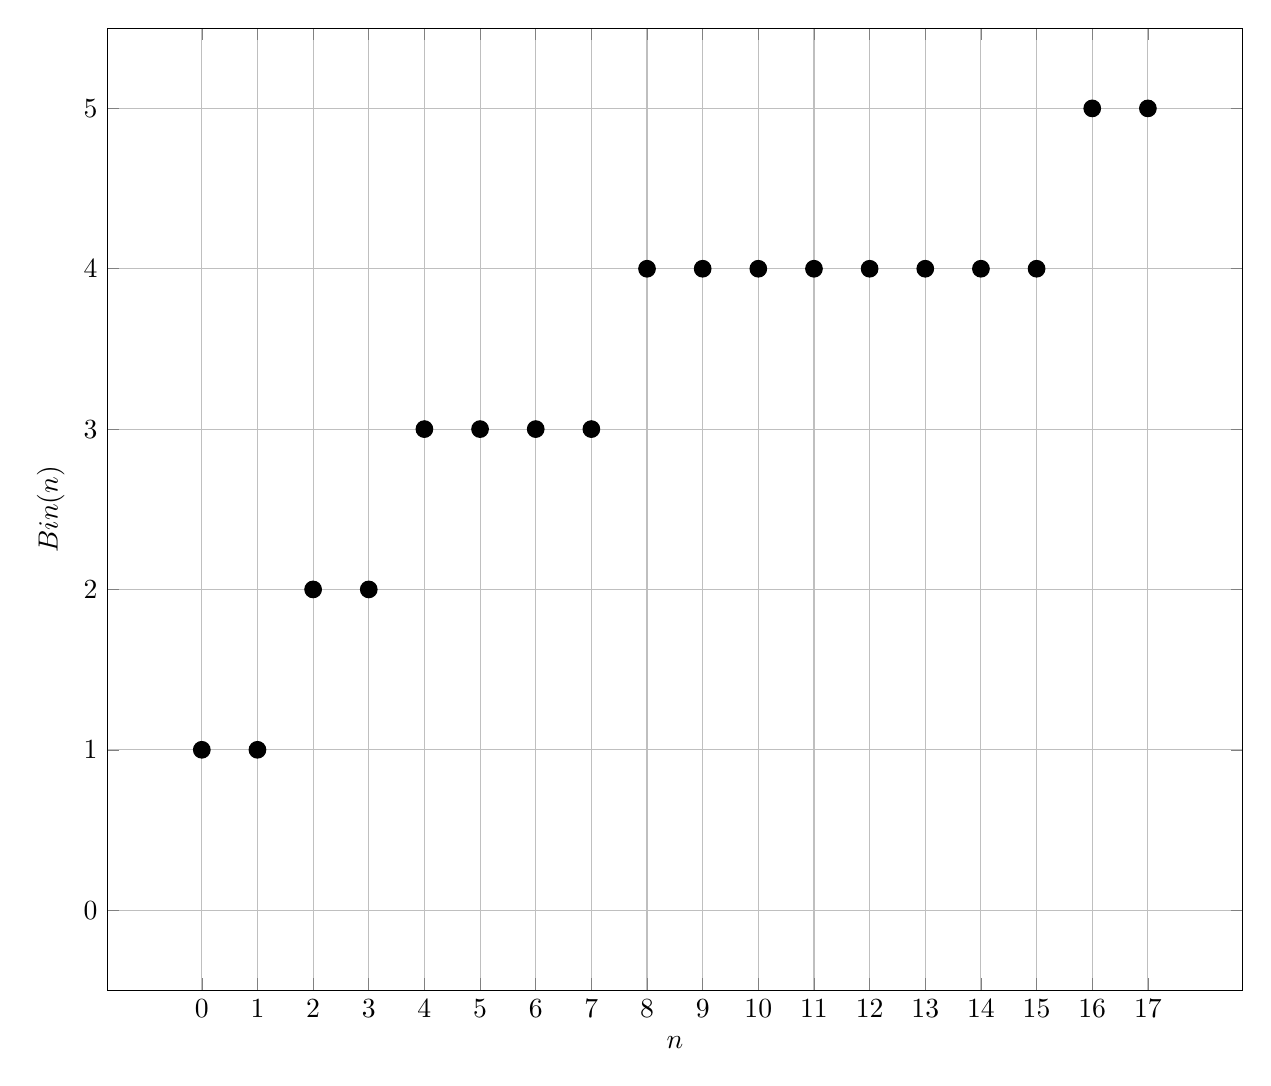
\begin{tikzpicture}
    \begin{axis}[
        width=16cm, % Adjust the width as desired
        domain=0:17,
        samples=18,
        xlabel={$n$},
        ylabel={$\text{Bin}(n)$},
        xtick={0, 1, 2, ..., 17},
        ytick={0, 1, ..., 5},
        grid=major,
        ymin=0, ymax=5,
        enlargelimits=true
    ]
    \addplot[
        only marks,
        mark=*,
        mark options={scale=1.5}
    ] table {
        x   y
        0   1  
        1   1
        2   2
        3   2
        4   3
        5   3
        6   3
        7   3
        8   4
        9   4
        10  4
        11  4
        12  4
        13  4
        14  4
        15  4
        16  5
        17  5
    };
    \end{axis}
\end{tikzpicture}
\end{figure}
\end{solution}


\question[2] Im Unterricht haben wir die Python \pythoninline{sieb} wie in \cref{listing:sieve} implementiert. 
Schreiben Sie eine Python-Funktion \pythoninline{def Prim(n)}, welche \pythoninline{sieb} verwendet um die Funktion $\text{Prim}(n)$ für eine gegebene natürliche Zahl $n$ zu berechnen.

\begin{lstlisting}[language=Python,caption=Sieb des Eratosthenes,numbers=none,label=listing:sieve]
def sieb(n):
    primzahlen = []
    nicht_gestrichen = (n + 1) * [True]

    i = 2
    while i <= n:
        if nicht_gestrichen[i]:
            primzahlen.append(i)
            j = 2 * i
            while j <= n:
                nicht_gestrichen[j] = False
                j += i
        i += 1
    return primzahlen
\end{lstlisting}

\begin{lstlisting}[numbers=none]
  Testfälle:

  Prim(4) sollte printen: 2
  Prim(20) sollte printen: 20
  Prim(21) sollte printen: 20
\end{lstlisting}

\question[3]

Ein Kommunikationsprotokoll hat eine Fehlerwahrscheinlichkeit von $r\in\io{0}{1}$. Wie oft muss das Protokoll mindestens wiederholt werden, bis die Fehlerwahrscheinlichkeit kleiner als $w$ ist. 

\question[3] Gegeben sind die beiden Datensätze
\begin{itemize}
  \item $x := 000000$ in Zürich und
  \item $y := 101010$ in Boston.
\end{itemize}
Berechnen Sie die exakte Wahrscheinlichkeit, dass das Kommunikationsprotokoll in diesem Fall falsch entscheidet.


\end{questions}
